\documentclass{beamer}
%\usetheme{Warsaw}
\usetheme{default}
\usepackage[utf8]{inputenc}
\usepackage{ragged2e}
\usepackage[brazilian]{babel}
%\usepackage[brazil]{babel}
%\usepackage[latin1]{inputenc}
\usepackage{graphicx}
\usepackage{subfig}
\usepackage{tikz}
%\usepackage{cite}
\usepackage{enumerate}
\usepackage{multicol}
\usepackage{scalefnt}
\usepackage{epstopdf}
\DeclareGraphicsExtensions{.pdf,.png,.eps}
\usepackage{psfrag}
\usepackage{pifont}
\newcommand{\cmark}{\ding{51}}%
\newcommand{\xmark}{\ding{55}}%

\newcommand{\Hi}{{\mathcal{H}}}
\newcommand{\R}{{\mathbb{R}}}
\newcommand{\G}{{\mathbb{G}}}
\newcommand{\E}{{\mathcal{E}}}

\theoremstyle{theorem}
\newtheorem{teo}{Teorema}[section]
\newtheorem{conj}{Conjectura}[section]
\newtheorem{lem}{Lema}[section]
\newtheorem{coro}{Corolário}[section]
\theoremstyle{definition}
\newtheorem{defi}{Definição}[section]
\newtheorem{exem}{Exemplo}[section]

\setbeamertemplate{footline}[frame number]%coloca numeração nos slides
% Dados para o slide inicial da apresentação. %
\title{MO826A/MC936A/MC931S \\ Tópicos Especiais em Sistemas de Informação \\ eHealth - Informática e Saúde \\ Professor: André Santanchè}
\author{Lucas Ismaily Bezerra Freitas\\Marcos Felipe de Menezes Mota}
\institute[IC]{Universidade Estudal de Campinas\\Instituto de Computação}
\date[Junho 2018]{20 de Junho de 2018}



\AtBeginSection[]
{
\frame{\frametitle{Agenda}\tableofcontents}
\begin{frame}<beamer>
\frametitle{Agenda}
\tableofcontents[currentsection,currentsubsection]
\end{frame}
}

%----------------------------------------------------------------------------------------------------------%
\begin{document}
% Slide inicial %
\begin{frame}[plain]
\titlepage
\end{frame}

%--------------------------------------------------------------------------------------------------------- %
\section{Introdução}
\begin{frame}
\frametitle{Introdução}
\begin{block}{Aterosclerose}
	\begin{itemize}
		\item<1-> Aterosclerose é uma doença vascular crônica e progressiva que normalmente manifesta-se na idade adulta ou idade avançada
		\item<2-> Muito comum, mais de 2 milhões casos por ano no Brasil
		\item<3-> O tratamento pode ajudar, mas essa doença não tem cura
		\item<4-> Requer um diagnóstico médico
		\item<5-> Crônico: pode durar anos ou a vida inteira
	\end{itemize}
\end{block}
\end{frame}

\begin{frame}
\frametitle{Introdução}
\begin{block}{Aterosclerose}
\end{block}
\begin{figure}[htbp]
	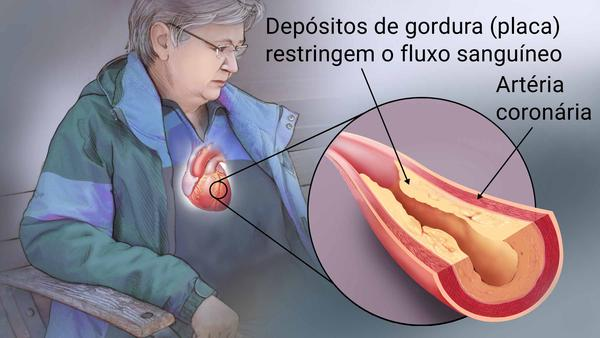
\includegraphics[scale=.45]{fig/fig1.jpeg}
\label{fig1}
\end{figure}
\end{frame}


%--------------------------------------------------------------------------------------------------------- %
\section{Definição do problema}
\begin{frame}
\frametitle{Problema}
\begin{block}{Sintomas da aterosclerose}
	\begin{itemize}
		\item<2-> Dilatações de algumas áreas dos vasos sanguíneos (aneurismas)
		\item<3-> Dor no peito tipo facada (angina ou infarto)
		\item<4-> Dores fortes na cabeça (derrame cerebral)
		\item<5-> Dores em braços e pernas (trombose)
		\item<6-> Dores no corpo
		\item<7-> Cansaço
	\end{itemize}
\end{block}

\begin{block}<8->{Exame Angio Tomografia de Coronárias}
	\begin{itemize}
		\item<9-> Custa em média 4,500 reais 
		\item<10-> Então, a ideia é tentar predizer a necessidade de realizar ou não o exame
	\end{itemize}
\end{block}


\end{frame}





%--------------------------------------------------------------------------------------------------------- %
\section{Técnica e Ferramenta escolhida}
\begin{frame}
\frametitle{Técnica e Ferramenta}
\begin{block}{Escolher a que tem o melhor resultado entre:}
	\begin{itemize}
		\item<2-> Redes Bayesiana 
		\item<3-> Floresta de decisão
		\item<4-> Árvore de decisão
	\end{itemize}
\end{block}

\begin{block}<5->{Ferramenta}
\begin{itemize}
\item Weka
\end{itemize}
\end{block}

\end{frame}


\section{Base de dados}
\begin{frame}
\frametitle{Base de dados}
\begin{block}{Base - aterosclerose}<2->
	\begin{itemize}
		\item<2-> Base com 14 atributos
		\item<3-> 303 instâncias
	\end{itemize}
\end{block}
\end{frame}

\begin{frame}
	\begin{figure}[htbp]
		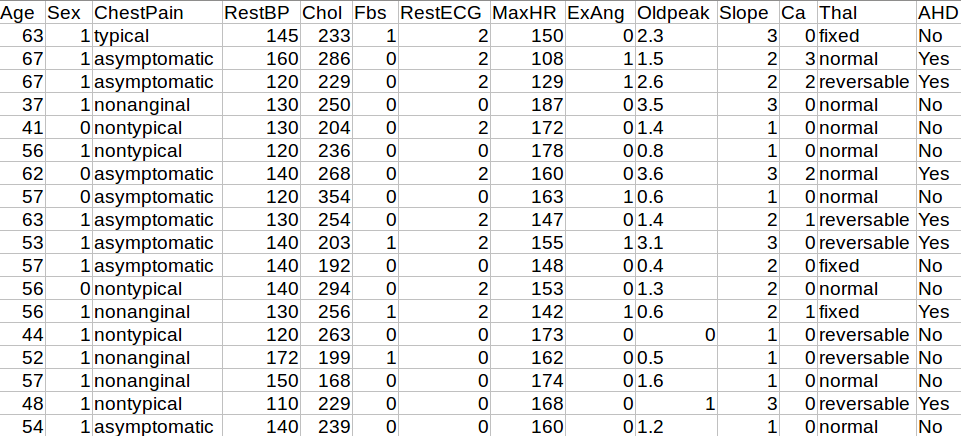
\includegraphics[scale=.30]{fig/Bd1.png}
		\caption{Dados de dados.}
	\end{figure}
\end{frame}

\begin{frame}
\frametitle{Base - aterosclerose}	

\begin{figure}[h]
\setcounter{subfigure}{0}
	\center
	\subfloat[]{
	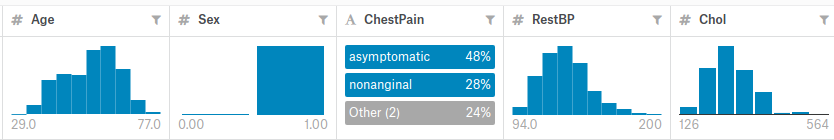
\includegraphics[scale=.38]{fig/descricao-1.png}
	}
	\pause
	\quad
	\subfloat[]{
	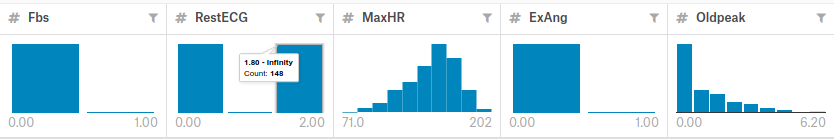
\includegraphics[scale=.38]{fig/descricao-2.png}
	}
	\pause
	\quad
	\subfloat[]{
	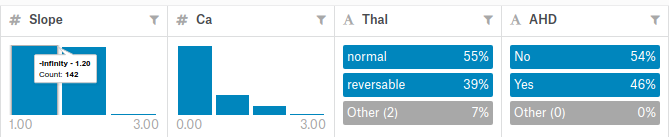
\includegraphics[scale=.38]{fig/descricao-3.png}
	}
	
\end{figure}
\end{frame}


%--------------------------------------------------------------------------------------------------------- %
\section{Resultados}

\begin{frame}
\frametitle{Resultados}
\begin{block}{Árvore de decisão}
\end{block}
\begin{figure}[htbp]
	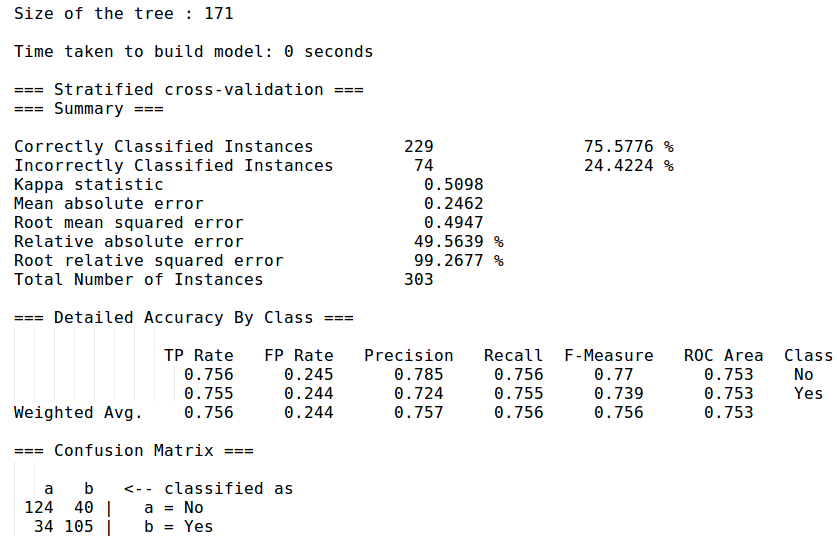
\includegraphics[scale=.35]{fig/result_tree.png}
\label{fig1}
\end{figure}
\end{frame}


\begin{frame}
\frametitle{Resultados}
\begin{block}{Floresta de decisão}
\end{block}
\begin{figure}[htbp]
	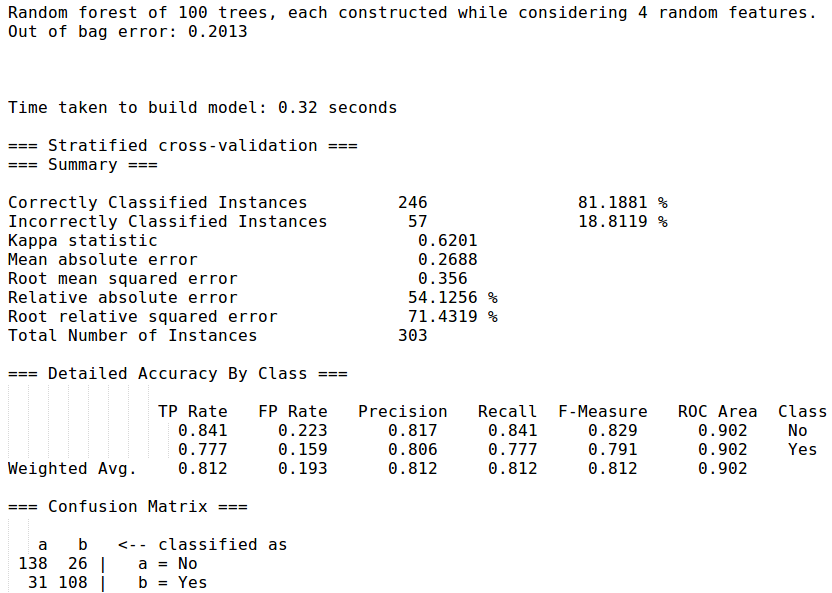
\includegraphics[scale=.35]{fig/result_forest.png}
\label{fig1}
\end{figure}
\end{frame}


\begin{frame}
\frametitle{Resultados}
\begin{block}{Rede Bayesiana}
\end{block}
\begin{figure}[htbp]
	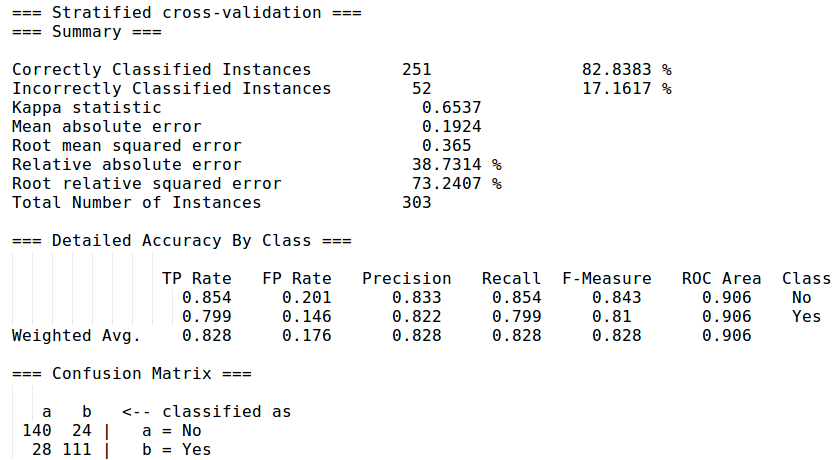
\includegraphics[scale=.35]{fig/result_bayse.png}
\label{fig1}
\end{figure}
\end{frame}

\begin{frame}
\frametitle{Resultados}
\begin{block}{Rede Bayesiana - Grafo}
\end{block}
\begin{figure}[htbp]
	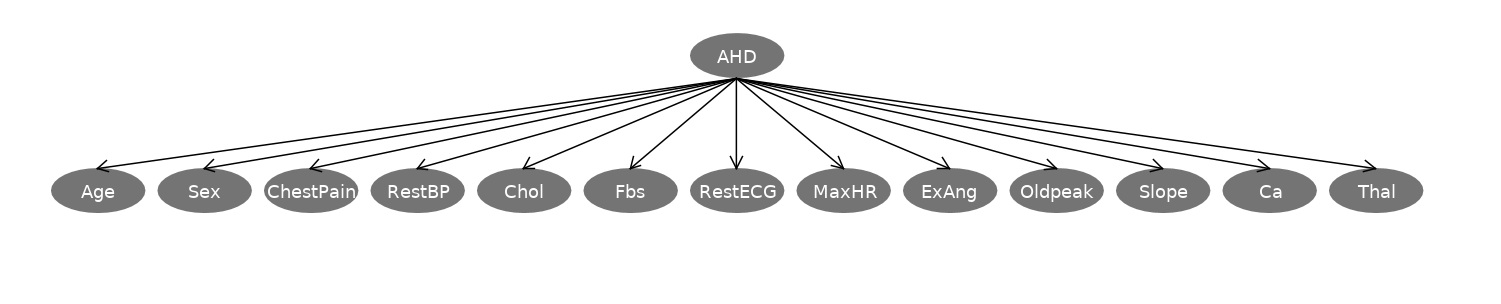
\includegraphics[scale=.23]{fig/BNK2.png}
\label{fig1}
\end{figure}
\end{frame}

\begin{frame}
\frametitle{Resultados}
\begin{block}{Escolher a que tem o melhor resultado entre:}
	\begin{itemize}
		\item Floresta de decisão \xmark
		\item Árvore de decisão \xmark
		\item Redes Bayesiana \cmark
	\end{itemize}
\end{block}

\begin{block}<2->{Atenção}
	\begin{itemize}
		\item Para esse conjunto de dados
		\item Cada contexto impõe restrições e dados diferentes
	\end{itemize}
\end{block}
\end{frame}


\begin{frame}
\frametitle{Resultados - Melhorando Redes Bayesianas}
\begin{block}{Rede Bayesiana - TAN}
\end{block}
\begin{figure}[htbp]
	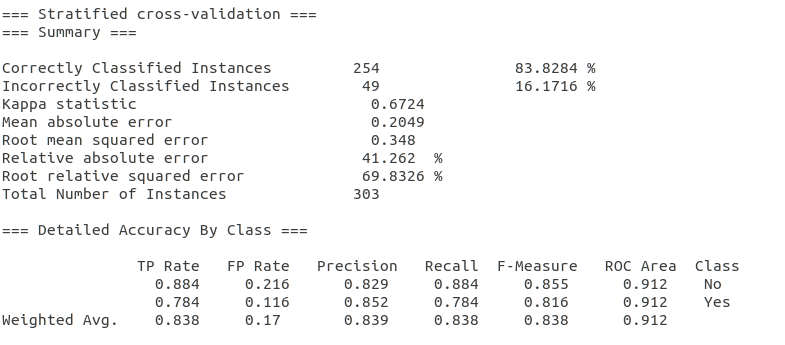
\includegraphics[scale=.35]{fig/BNAT-res.png}
\label{fig1}
\end{figure}
\end{frame}

\begin{frame}
\frametitle{Resultados - Melhorando Redes Bayesianas}
\begin{block}{Rede Bayesiana - TAN}
\end{block}
\begin{figure}[htbp]
	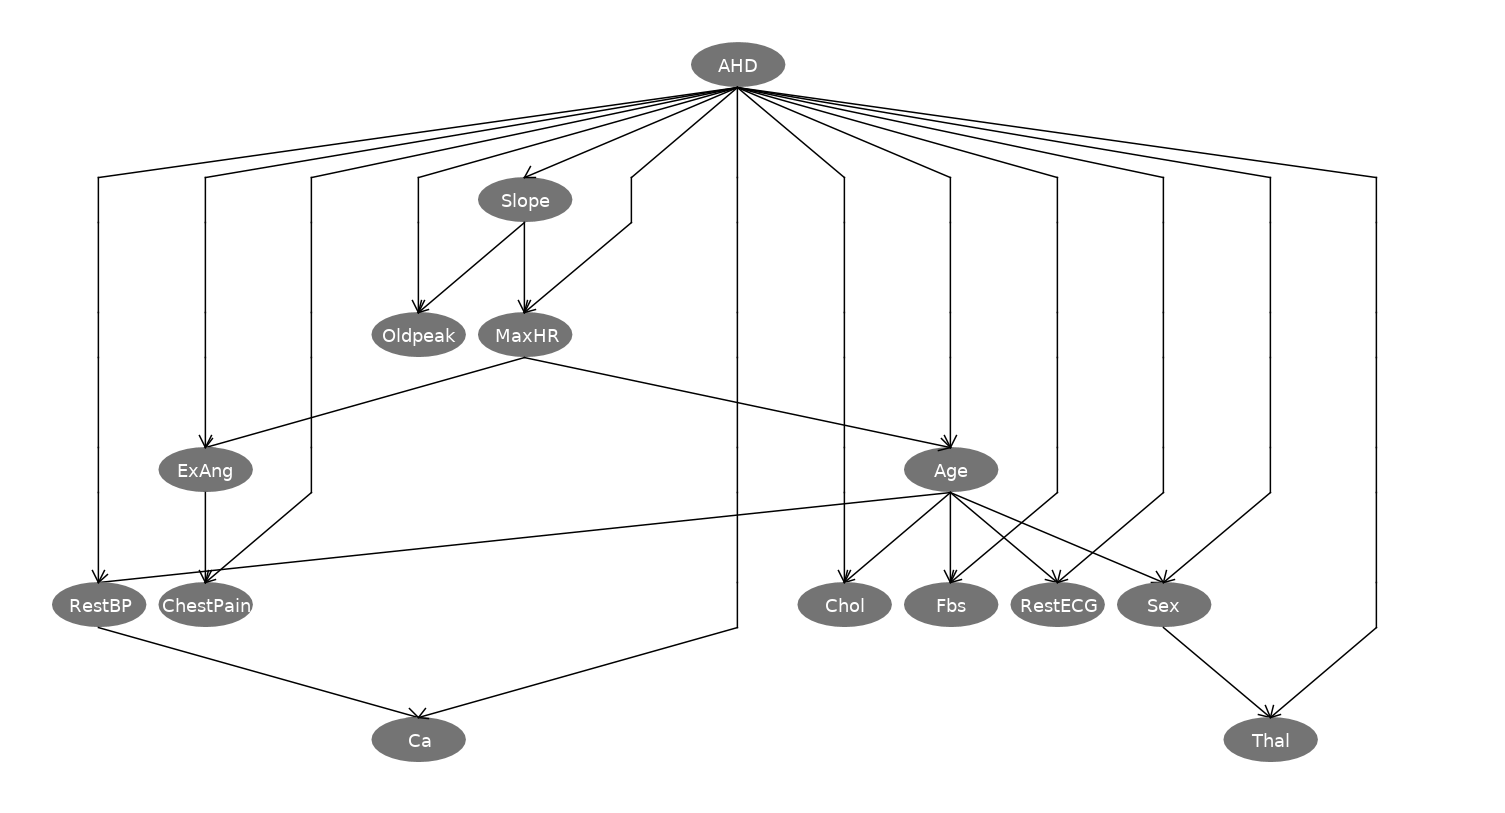
\includegraphics[scale=.21]{fig/BNAT-grafo.png}
\label{fig1}
\end{figure}
\end{frame}

\begin{frame}
\frametitle{Resultados - Melhorando Redes Bayesianas}
\begin{block}{Rede Bayesiana - Inductive Causation}
\end{block}
\begin{figure}[htbp]
	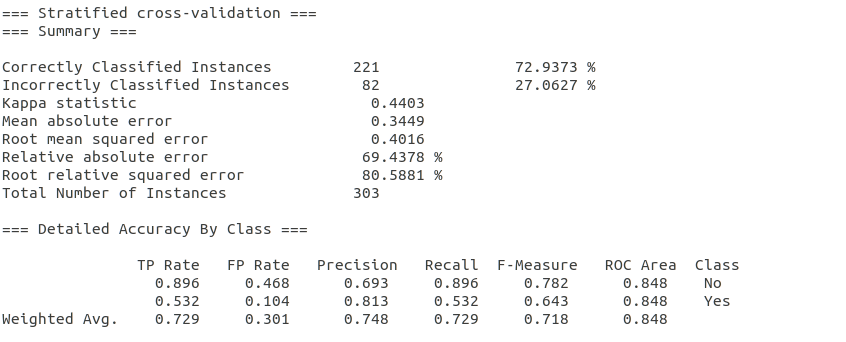
\includegraphics[scale=.35]{fig/BNIC-res.png}
\label{fig1}
\end{figure}
\end{frame}

\begin{frame}
\frametitle{Resultados - Melhorando Redes Bayesianas}
\begin{block}{Rede Bayesiana - Inductive Causation}
\end{block}
\begin{figure}[htbp]
	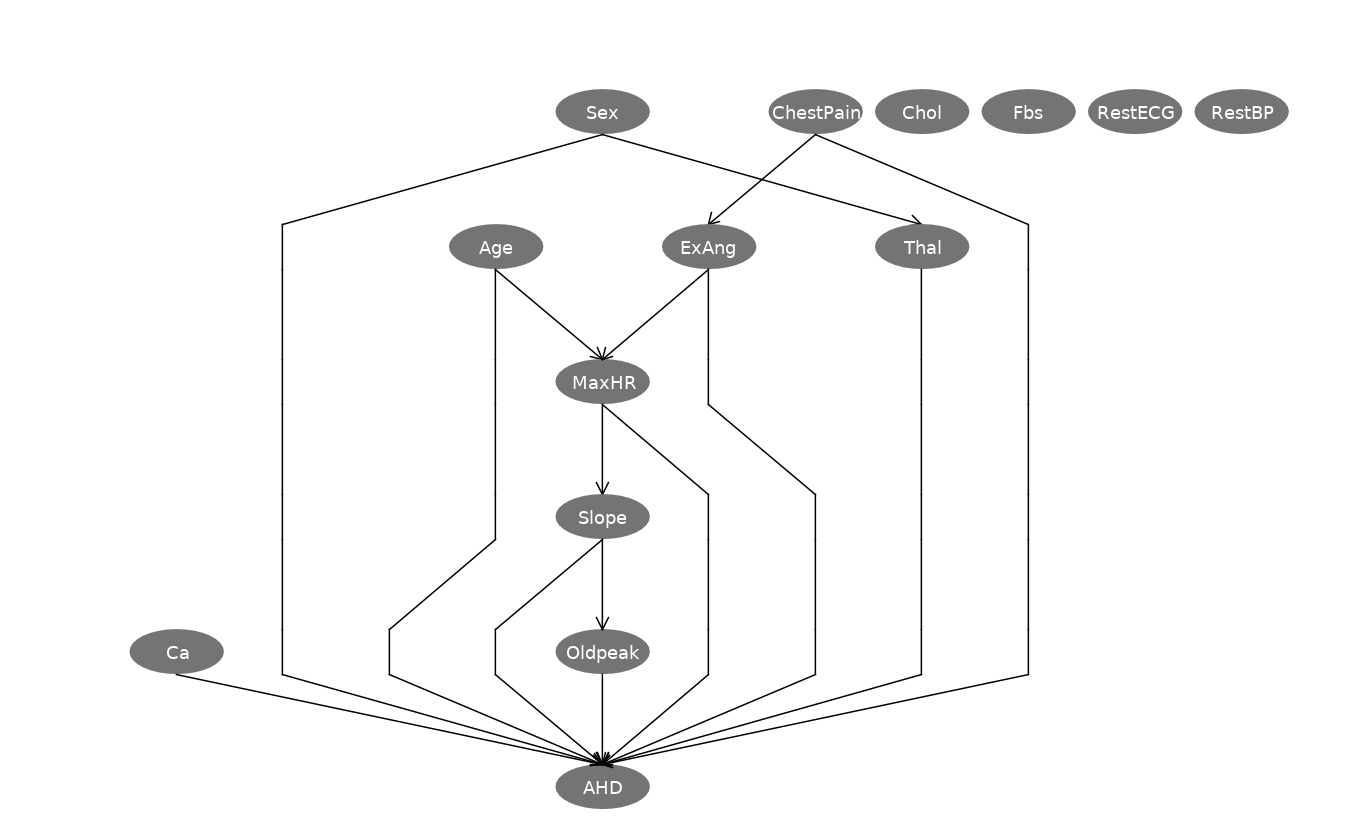
\includegraphics[scale=.21]{fig/BNIC-grafo.png}
\label{fig1}
\end{figure}
\end{frame}


\begin{frame}
\frametitle{Dúvidas?}	
\begin{figure}[htbp]
		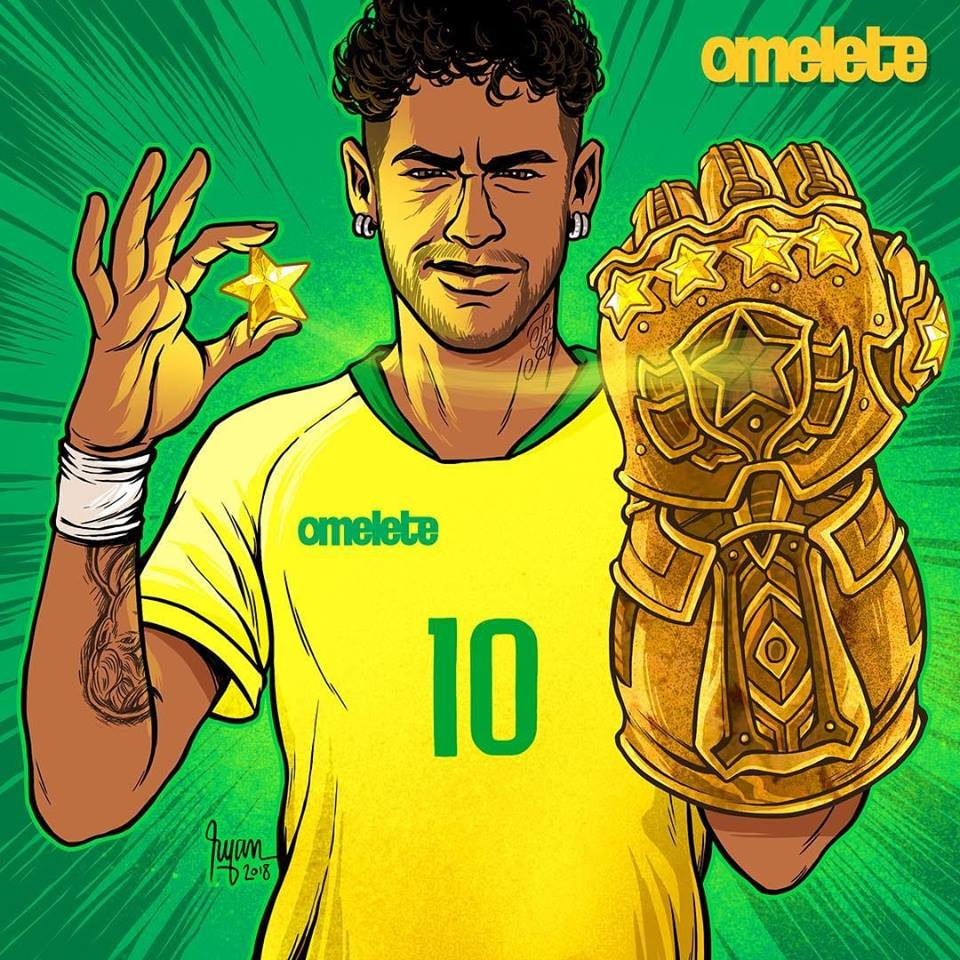
\includegraphics[scale=.25]{fig/ney.jpg}
\end{figure}
\end{frame}

\end{document}


